\documentclass[10pt]{standalone}
\usepackage{amsmath}
\usepackage{pgf,tikz}
\usetikzlibrary{shapes,arrows}
\usepackage{mathrsfs}
\usepackage{amsmath, amsthm, amssymb}   
\usetikzlibrary{arrows}
\pagestyle{empty}
\begin{document}
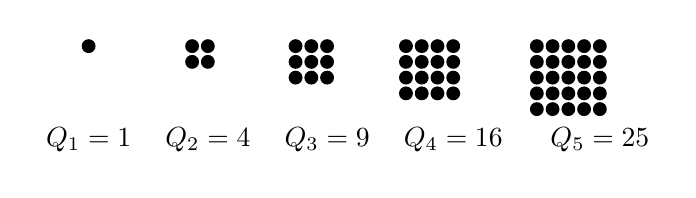
\begin{tikzpicture}[node distance=0.2cm]
%\tikzset{
%	tondo/.style={draw, circle, minimum size=.1cm, node distance=0.35cm,fill=green}
%}
% \matrix[row sep=0.cm,column sep=0.3cm] {
% 	\node  [tondo](A){}; 
% 	&
% 	\node   [tondo,left of=A](B) {};
% 	\node[tondo,below of=B](B1) {};     
% 	\node[tondo,right of=B1](B2) {};
% 	     &
% 	\node  [tondo,left of=B](C){};
% 	\node  [tondo,below of=C](C1){}; 
% 	\node  [tondo,right of=C1](C2){}; 
% 	\node  [tondo,below of=C1](C3){}; 
% 	\node  [tondo,right of=C3](C4){}; 
% 	\node  [tondo,right of=C4](C5){}; 
% 		     &
% 	\node  [tondo,left of=C](D){};
% 	\node  [tondo,below of=D](D1){}; 
% 	\node  [tondo,right of=D1](D2){}; 
% 	\node  [tondo,below of=D1](D3){}; 
% 	\node  [tondo,right of=D3](D4){}; 
% 	\node  [tondo,right of=D4](D5){}; 
% 	\node  [tondo,below of=D3](D6){}; 
% 	\node  [tondo,right of=D6](D7){}; 
% 	\node  [tondo,right of=D7](D8){}; 
% 	\node  [tondo,right of=D8](D9){}; 
% 	\\
% 	\node  (R1){$T_1=1$}; 	&\node  (R2){$T_2=3$}; &\node  (R3){$T_3=6$}; &\node  (R4){$T_4=10$}; \\
% 	};
 \matrix[row sep=0.0cm,column sep=0.2cm] {
	\node  (A){}; 
	&
	\node   [left of=A](B) {};
	\node[below of=B](B1) {};     
	\node[right of=B1](B2) {};
	\node[right of=B](B3) {};
	&
	\node  [left of=B](C){};
	\node  [below of=C](C1){}; 
	\node  [right of=C1](C2){}; 
	\node  [below of=C1](C3){}; 
	\node  [right of=C3](C4){}; 
	\node  [right of=C4](C5){}; 
	\node  [right of=C](C6){};
	\node  [right of=C2](C7){};
	\node  [right of=C6](C8){};
	&
	\node  [left of=C](D){};
	\node  [right of=D](D1){}; 
	\node  [right of=D1](D2){}; 
	\node  [right of=D2](D3){}; 
	\node  [below of=D](D4){}; 
	\node  [right of=D4](D5){}; 
	\node  [right of=D5](D6){}; 
	\node  [right of=D6](D7){}; 
	\node  [below of=D4](D8){}; 
	\node  [right of=D8](D9){}; 
	\node  [right of=D9 ](D10){};
	\node  [right of=D10](D11){};
	
	\node  [below of=D8](D12){};
	\node  [right of=D12](D13){};
	\node  [right of=D13](D14){}; 
	\node  [right of=D14](D15){};
		&
	\node  [left of=D](E){};
	\node  [right of=E](E1){}; 
	\node  [right of=E1](E2){}; 
	\node  [right of=E2](E3){}; 
	\node  [right of=E3](E4){}; 
	\node  [below of=E](E5){}; 
	\node  [right of=E5](E6){}; 
	\node  [right of=E6](E7){}; 
	\node  [right of=E7](E8){}; 
	\node  [right of=E8](E9){}; 
	\node  [below of=E5](E10){}; 
	\node  [right of=E10](E11){}; 
	\node  [right of=E11](E12){}; 
	\node  [right of=E12](E13){};
	\node  [right of=E13](E14){};
	\node  [below of=E10](E15){}; 
	\node  [right of=E15](E16){}; 
	\node  [right of=E16](E17){}; 
	\node  [right of=E17](E18){};
	\node  [right of=E18](E19){};
	\node  [below of=E15](E20){}; 
	\node  [right of=E20](E21){}; 
	\node  [right of=E21](E22){}; 
	\node  [right of=E22](E23){};
	\node  [right of=E23](E24){};
	\\
	\node  (R1){$Q_1=1$}; 	&\node  (R2){$Q_2=4$}; &\node  (R3){$Q_3=9$}; &\node  (R4){$Q_4=16$}; &\node  (R5){$Q_5=25$};\\
};
\fill (A) circle [radius=2.5pt];
\fill (B) circle [radius=2.5pt];
\fill (B1) circle [radius=2.5pt];
\fill (B2) circle [radius=2.5pt];
\fill (B3) circle [radius=2.5pt];
\fill (C) circle [radius=2.5pt];
\fill (C1) circle [radius=2.5pt];
\fill (C2) circle [radius=2.5pt];
\fill (C3) circle [radius=2.5pt];
\fill (C4) circle [radius=2.5pt];
\fill (C5) circle [radius=2.5pt];
\fill (C6) circle [radius=2.5pt];
\fill (C7) circle [radius=2.5pt];
\fill (C8) circle [radius=2.5pt];
\fill (D) circle [radius=2.5pt];
\fill (D1) circle [radius=2.5pt];
\fill (D2) circle [radius=2.5pt];
\fill (D3) circle [radius=2.5pt];
\fill (D4) circle [radius=2.5pt];
\fill (D5) circle [radius=2.5pt];
\fill (D6) circle [radius=2.5pt];
\fill (D7) circle [radius=2.5pt];
\fill (D8) circle [radius=2.5pt];
\fill (D9) circle [radius=2.5pt];
\fill (D10) circle [radius=2.5pt];
\fill (D11) circle [radius=2.5pt];
\fill (D12) circle [radius=2.5pt];
\fill (D13) circle [radius=2.5pt];
\fill (D14) circle [radius=2.5pt];
\fill (D15) circle [radius=2.5pt];
\fill (E) circle [radius=2.5pt];
\fill (E1) circle [radius=2.5pt];
\fill (E2) circle [radius=2.5pt];
\fill (E3) circle [radius=2.5pt];
\fill (E4) circle [radius=2.5pt];
\fill (E5) circle [radius=2.5pt];
\fill (E6) circle [radius=2.5pt];
\fill (E7) circle [radius=2.5pt];
\fill (E8) circle [radius=2.5pt];
\fill (E9) circle [radius=2.5pt];
\fill (E10) circle [radius=2.5pt];
\fill (E11) circle [radius=2.5pt];
\fill (E12) circle [radius=2.5pt];
\fill (E13) circle [radius=2.5pt];
\fill (E14) circle [radius=2.5pt];
\fill (E15) circle [radius=2.5pt];
\fill (E16) circle [radius=2.5pt];
\fill (E17) circle [radius=2.5pt];
\fill (E18) circle [radius=2.5pt];
\fill (E19) circle [radius=2.5pt];
\fill (E20) circle [radius=2.5pt];
\fill (E21) circle [radius=2.5pt];
\fill (E22) circle [radius=2.5pt];
\fill (E23) circle [radius=2.5pt];
\fill (E24) circle [radius=2.5pt];
\end{tikzpicture}
    
\end{document}